\chapter{Experimentación}\label{chapter:implementation}

En el capítulo se describen los conjuntos de datos utilizados para el entrenamiento y validación del modelo 
propuesto y cómo se construyen los conjuntos de datos en español. Se mencionan las herramientas utilizadas 
para la confección del software. Además, se describe el 
proceso de experimentación y evaluación de los modelos construídos con los conjuntos de datos. Finalmente,
se presentan los resultados obtenidos al aplicarles los modelos a las Cartas a la Dirección extraídas 
del periódico Granma. 

\section{Conjuntos de Datos}

Para el entrenamiento de los modelos propuestos se utilizaron corpus diferentes, estos
presentan esquemas de anotación distintos entre sí, difieriendo principalmente en la definición de UDA y 
las clasificaciones dadas a estas y a las relaciones. A todos los conjuntos se les proyectó al lenguaje 
español y se les realizó un aumento de datos. Como conjunto para la validación fueron usadas 
una parte de las Cartas a la Dirección del periódico Granma.

\subsection{Ensayos Argumentativos}\label{corpus:persuasive_essays}

Este corpus [\cite{stab2017parsing}] presenta unos 402 documentos, dividido por los autores en 286 documentos para entrenamiento (70\%), 
80 para prueba (20\%) y 36 para validación (10\%). Los contenidos de estos son ensayos de estudiantes en los que 
se argumentan sobre temas como cooperar o competir y contribuciones de la tecnología a la sociedad.
Las anotaciones de las UDAs se conforman por segmentos de textos argumentativos, estos segmentos son 
clasificados en \emph{MajorClaim} (751, 12\%), \emph{Claim} (1506, 25\%) y \emph{Premise} (3832, 63\%).
La estructura de las relaciones entre las UDAs conforman árboles en los que se tienen como raíz las 
\emph{MajorClaim} del texto. Las relaciones solo están permitidas entre \emph{Premise-Premise} y \emph{Premise-Claim}, clasificadas
en \emph{attack} (219, 6\%) y \emph{support} (3613, 94\%). Las relaciones entre \emph{Claim} y \emph{MajorClaim} son anotadas 
de manera diferente, por medio de 
darle a las \emph{Claim} una clasificación de si está a favor (1228) o en contra (278) de las \emph{MajorClaim} del documento.
Para el análisis de este corpus se consideraron las relaciones \emph{Claim-MajorClaim} de igual manera que las otras,
al convertir estas posiciones en relaciones. El número final con la inclusión de estas aumenta a 715 (10\%) de ataque y 
5958 (90\%) de apoyo.

\subsection{CDCP}\label{corpus:cdcp}

El corpus [\cite{niculae2017argument}] está conformado por 731 comentarios de usuarios extraídos de la web bajo el tema de 
prácticas de cobro de deudas a los consumidores (CDCP en inglés).
Las UDAs se encuentran segmentadas en oraciones y todas se consideran argumentativas, estas son clasificadas en 
\emph{policy} (815, 17\%), \emph{value} (2180, 45\%), \emph{fact} (785, 16\%), \emph{testimony} (1116, 21\%) y \emph{reference} (32 1\%). 
Las relaciones se encuentran clasificadas en \emph{reason} (1352, 97\%) y \emph{evidence} (73, 3\%).

\subsection{AbsTRCT}

AbsTRCT [\cite{mayer2020transformer}] se compone de 500 documentos sobre el estudio de cuatro enfermedades diferentes,
glaucoma, hipertensión, hepatitis b y diabetes. Las UDAs constituyen oraciones, aunque no todas son consideradas
argumentativas. Estas se clasifican en \emph{MajorClaim} (93, 3\%), \emph{Claim} (993, 30\%) y \emph{Premise} (2198, 67\%).
Las relaciones están representadas por tres categorías: \emph{support} (1763, 85\%), \emph{partial-attack} (238, 12\%) y
\emph{attack} (60, 3\%).

En resumen, estos datos no son grandes y contiene una gran cantidad de desbalance en sus clases.
En la Tabla \ref{table:corpus_info} se muestran los datos promedio de la composición de los diferentes corpus. 
Se observa una composición heterogenea entre estos, principalmente CDCP difiere en gran número de los demás.

\begin{table}[h!]
	\begin{center}
		\scalebox{0.8}{
		\begin{tabular}{|c|c|c|c|c|} \hline
		Corpus		            & Tokens 	& Tokens argumentativos	& UDAs   & Relaciones por UDA    \\ \hline
		Ensayos Argumentativos  & 381		& 68\% 					& 35\% 	 & 1,08					 \\ \hline
		CDCP		            & 127		& 99\% 					& 97\% 	 & 0,30					 \\ \hline
		AbsTRCT	                & 371		& 50\% 					& 47\% 	 & 0,63					 \\ \hline
		\end{tabular}
		}
	\caption{Información de promedios de los conjuntos de datos.}\label{table:corpus_info}
	\end{center}
\end{table}

\subsection{Creación de corpus en español}

\subsubsection{Aumento de datos}

% TODO PREGUNTAR Dice poner {back-translation} aunque en la referencia original lo dice junto
A los conjuntos de datos a analizar se les realizó un aumento de datos mediante le técnica de \emph{backtranslation},
aplicándole la proyección de etiquetas de los elementos originales a los aumentados.
Esto contribuyó a duplicar la cantidad de elementos disponibles. Los resultados obtenidos al comparar los 
elementos originales con los aumentados se reflejan en la Tabla \ref{table:data_augmentation}.
Estos muestran que se logró una variación pequeña en los datos, aunque conservando la 
longitud original del texto. 

\begin{table}[h!]
	\begin{center}
		\scalebox{1}{
		\begin{tabular}{|c|c|c|c|c|} \hline
		Corpus		            &  Jaccard	& Levenshtein	& $\frac{|\mathrm{Palabras} \quad \mathrm{originales}|}{|\mathrm{Palabras \quad aumentadas}|}$   \\ \hline
        Ensayos Argumentativos	&  0.69		                & 96		                    & 1.00	  \\ \hline
		CDCP                    &  0.72	                    & 30		                    & 1.02	  \\ \hline
        AbsTRCT                 &  0.74		                & 86		                    & 1.04	  \\ \hline
		\end{tabular}
		}
	\caption{Datos promedios comparando los textos originales con los aumentados.}\label{table:data_augmentation}
	\end{center}
\end{table}

\subsubsection{Proyección de corpus}

Todos los conjuntos de datos están originalmente en inglés, por lo tanto, se les aplicó el algoritmo de proyección
de corpus para obtener uno en español para ser usado en el entrenamiento de los modelos. 
Para la traducción automática se utilizó el servicio de Google Translate\footnote{\href{https://translate.google.com/}{https://translate.google.com/}}. 
Para calcular las 
alineaciones de palabras se probaron dos algoritmos: FastAlign [\cite{dyer2013fastalign}] y AwesomeAlign 
[\cite{dou2021word}]. Se observó que el primero, aunque es más rápido posee una calidad menor en los resultados,
el segundo posee una mayor calidad, aunque requiere de mayor tiempo y recursos para ejecutarse. Para los experimentos
se usó finalmente AwesomeAlign. La proyección de las etiquetas fue llevada a cabo por el algoritmo propuesto 
% TODO Cite problem, citar como texto
% [\autocite{eger2018cross}] 
% [\parencite{eger2018cross}] 
% [\citet{eger2018cross}] 
% [\citep{eger2018cross}] 
en \textcite{eger2018cross}.

\subsection{Cartas a la Dirección}

Las Cartas a la Dirección constituyen un segmento del periódico Granma donde son publicadas
cartas enviadas por la población o empresas a dicha entidad. En general, las cartas 
presentan dudas o problemas de la población con el objetivo de obtener respuestas del organismo
asociado. Se extrajeron 2891 cartas desde el 30 de agosto del 2013 hasta el 28 de octubre del 2022. Estas 
contienen aproximadamente 975000 palabras en los datos, en promedio, la cantidad de palabras por carta es de 330.
Se encontraron 874 cartas en respuesta a cartas enviadas, lo que representa un 30\% del total. Se extrajeron
los comentarios asociados a las cartas, en este sentido 987 cartas no presentan comentarios y, en promedio, 
se realizan 2 comentarios por carta. Los textos presentan un título y un formato relativamente libre, 
aunque en las cartas de respuesta se puede observar una firma de la persona que respondió y la entidad que 
representa. Del total de cartas, se seleccionaron las que fueran en respuesta a otra y también las 
cartas que fueron respondidas para tener una mayor concentración de cartas que fueran argumentativas, 
esta selección está conformada por 1702 cartas, lo que representa un 59\% del total de cartas.

\section{Implementación}

La implementación de los modelos y algoritmos de procesamiento y visualización de datos se encuentran en 
un repositorio de GitHub\footnote{\url{https://github.com/luisoibarra/argument-mining}}. Esta implementación
está concebida para que se pueda extender fácilmente para el uso con otros idiomas diferentes del inglés y el 
español. Se basa en una arquitectura de procesamiento secuencial en el cual cada paso del proceso realiza
una tarea específica y lo más desacoplada posible de las otras. Las tareas realizadas son:

\begin{itemize}
    \item Creación del corpus en un formato estándar: dado que los corpus vienen en diferentes 
	formas, este paso se realiza para trabajar sobre una misma representación de este.
    \item Proyección del corpus de un lenguaje fuente a un lenguaje objetivo: en el caso de 
	uso del trabajo se proyecta del inglés al español.
    \begin{itemize}
        \item Traducción y alineación de oraciones.
        \item Alineación de palabras.
        \item Proyección de etiquetas.
    \end{itemize}
    \item Extracción y clasificación de UDAs.
    \item Extracción y clasificación de las relaciones entre las UDAs.
    \item Visualización de los resultados.
\end{itemize}

\subsection{Herramientas}

El lenguaje empleado para la confección del software fue Python [\cite{python}], este presenta 
una gran variedad de herramientas 
para el trabajo con texto, visualización de datos y creación de modelos de aprendizaje profundo.
Se utilizó tensorflow [\cite{tensorflow}] en su versión 2.9.2 para la construcción y entrenamiento de los modelos. 
Para el procesamiento de los textos se utilizaron nltk [\cite{nltk}] y spacy [\cite{spacy}], con estos se realizaron tareas
como la extracción de tokens y oraciones del texto, la anotación de las etiquetas de partes de la oracion. Se utilizaron 
ambos paquetes para el procesamiento debido a que, en dependencia de la situación, cada uno presenta diferentes
ventajas. En el caso de nltk, presenta algoritmos rápidos para el procesamiento de texto que no 
requieren de muchos recursos computacionales, sin embargo, estos algoritmos no están disponibles de inmediato
para otros lenguajes como el español. Spacy por su parte presenta algoritmos más certeros a costo 
de mayor tiempo de procesamiento y gasto de recursos computacionales, y también presenta una cantidad mayor de lenguajes 
disponibles. Para la visualización y manejo de los datos, y cálculo de métricas se utilizaron 
matplotlib [\cite{matplotlib}], pandas [\cite{pandas}] y sklearn [\cite{sklearn}]. 
Para la recolección de las Cartas a la Dirección del periódico Granma se utilizó scrapy [\cite{scrapy}].
Como interfaz visual para el usuario se utilizó la herramienta Brat [\cite{brat}] 
(Figura \ref{fig:brat_persuasive_granma_letters}). Esta herramienta permite
la visualización y edición de las estructuras argumentativas. Dado que Brat es una página web, esta se puede
desplegar y permite su uso online.

\begin{figure}[h!]
	\begin{center}
		% 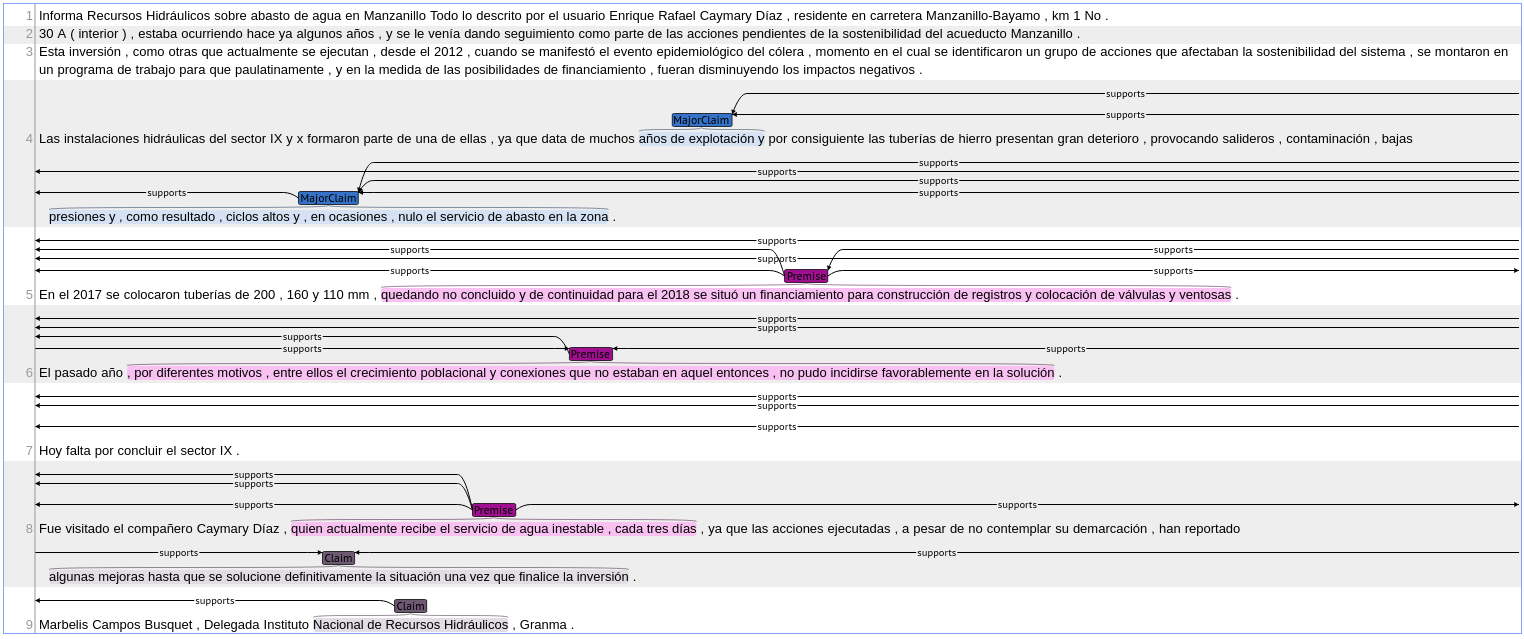
\includegraphics[scale=.4]{Graphics/persuasive_2019-01-25|informa-recursos-hidraulicos-sobre-abasto-de-agua-en-manzanillo|abasto-de-agua-en-manzanillo.png}
		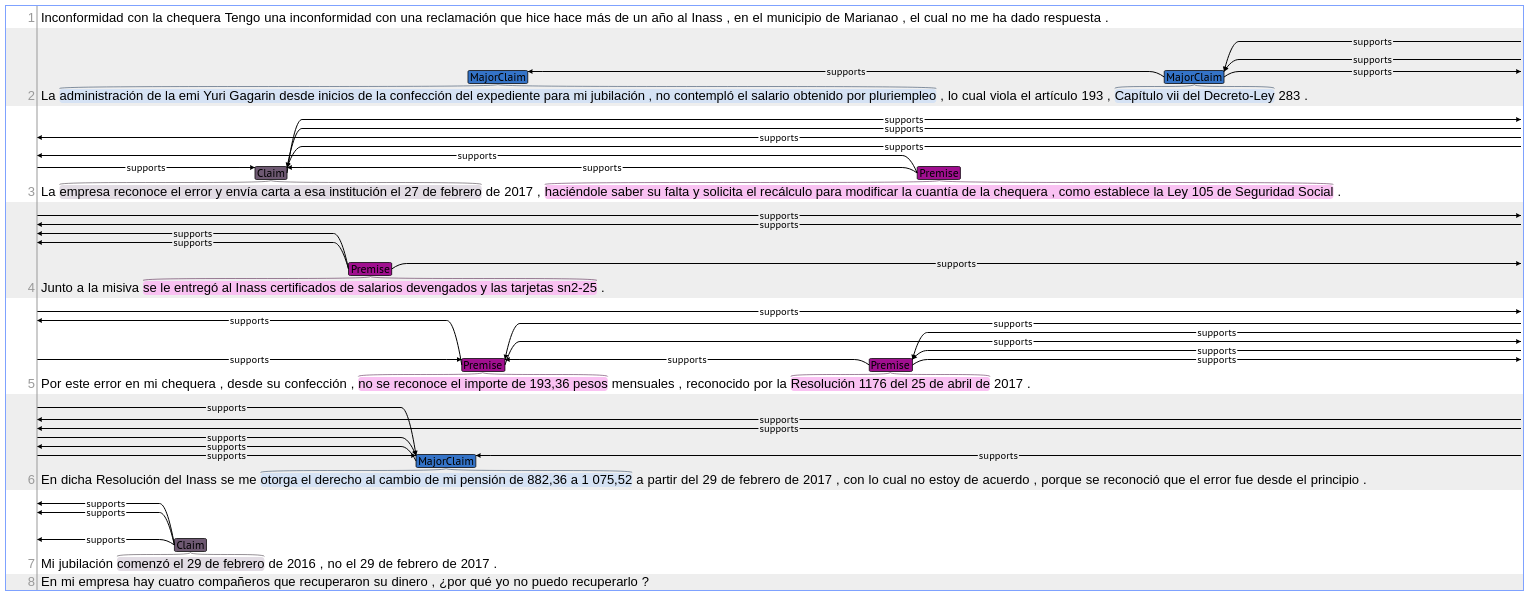
\includegraphics[scale=.4, width=435pt, height=250pt]{Graphics/persuasive_2019-03-22|inconformidad-con-la-chequera.png}
		\caption{Visualización con Brat de las estructuras argumentativas.}\label{fig:brat_persuasive_granma_letters}
	\end{center}
\end{figure}

\subsection{Formato Estándar}

El formato estándar creado es basado en el esquema de anotación CoNLL, donde se anotan a nivel de token todos los aspectos 
relavantes para las tareas a realizar. La segmentación de las UDAs son representadas por las anotaciones 
BIO o BIOES en cada palabra, en adición, las clasificaciones de estas son anotadas al adicionar el nombre 
de esta separada por un guión. Las relaciones son anotadas auxiliándose de la distancia argumentativa, estas 
son agregadas al anotar el tipo de relación con su respectiva distancia ambas separadas por un guión. A 
continuación se muestran ejemplos de este formato, conformado por el token, su clasificación BIOES, su clasificación
UDA, y las relaciones representadas por su clasificación y su distancia argumentativa:

\begin{itemize}
	\item Elemento fuera de una UDA: $análisis \quad O$
	\item UDA intermedia con una relación: $contribuye \quad I-Premise-attacks-5$
	\item Inicio de UDA con dos relaciones: $atletas \quad B-Claim-attacks--1-attacks-12$
\end{itemize}

\section{Experimentación}

Para realizar la selección del modelo se utilizó el corpus de Ensayos Argumentativos. Con este se ajustaron
las arquitecturas e hiperparámetros de los modelos propuestos. La mejor combinación de estos fue utilizada 
para el entrenamiento de los corpus restantes. Finalmente, los modelos fueron utilizados para anotar las Cartas 
a la Dirección. 

\subsection{Hardware}

Gran parte del procesamiento se llevo a cabo en una computadora $i5$ con $8GB$ de RAM ampliada con $4GB$ de memoria 
\emph{swap} [\cite{swap}], aunque se requirió el uso de la plataforma Colab [\cite{colab}] para 
el entrenamiento de algunos modelos por falta de recursos locales.

\subsection{Segmentador de UDA}

En el entrenamiento del segmentador de UDA se hicieron variaciones en la arquitectura propuesta con respecto a la
presencia o no de las siguientes componentes, presentando cuatro candidatos (Tabla \ref{table:segmenter_architecture_table}):

\begin{itemize}
    \item Atributos de POS en la entrada del algoritmo (POS).
    \item Atributos extraídos por la CNN de la palabra (Char-CNN).
    \item Atributos extraídos por la LSTM bidireccional de la palabra (Char-LSTM).
    \item Conexiones residuales (Res).
    \item Capa densa final (Densa).
    \item Capas de normalizaciones (Norm).
\end{itemize}

\begin{table}[h!]
	\begin{center}
		\begin{tabular}{|c|c|c|c|c|c|c|} \hline
		Modelos 		& POS       & Char-CNN  & Char-LSTM & Res       & Norm      & Densa  \\ \hline
		Modelo 1		& $\times$	& $\times$    & $\times$    & $\times$	& $\times$    & $\times$ \\ \hline
		Modelo 2		& $\times$	& $\checkmark$    & $\checkmark$    & $\checkmark$	& $\checkmark$    & $\times$ \\ \hline
		Modelo 3		& $\checkmark$	& $\checkmark$    & $\checkmark$    & $\checkmark$	& $\checkmark$    & $\times$ \\ \hline
		Modelo 4		& $\checkmark$	& $\checkmark$    & $\checkmark$    & $\checkmark$	& $\checkmark$    & $\checkmark$ \\ \hline
		\end{tabular}
	\caption{Variantes de arquitectura de los modelos de segmentación de UDA.}\label{table:segmenter_architecture_table}
	\end{center}
\end{table}

En la Figura \ref{fig:segmenter_model_loss} se observan las diferentes curvas de aprendizaje de los modelos 
probados. Se muestra la rápida convergencia de los modelos con conexiones residuales y normalizaciones.
Se muestra también la tendencia al sobreajuste en el entrenamiento entre los pasos 17-20, en donde se detiene el 
entrenamiento para evitar el crecimiento del error de generalización.

\begin{figure}[h!]
	\begin{center}
		\begin{center}
			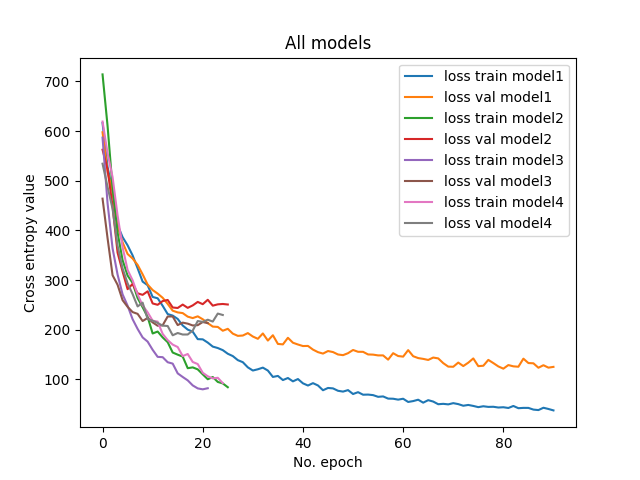
\includegraphics[scale=.7]{Graphics/persuasive_essays_all_linked_crf_loss.png}
        \end{center}
	    \caption{Pérdida de los modelos segmentadores.}\label{fig:segmenter_model_loss}
	\end{center}
\end{figure}

Las métricas 100\%F1 y 50\%F1 muestran que los modelos 1 y 2 presentan un desempeño menor que los 3 y 4. 
Se muestra un ligero aumento de 1\% en las 50\%F1 en el modelo 4 con respecto 
al modelo 3, aunque las métricas de F1 en el 3 superan a las de 4. Se considera a la 
segmentación como tarea principal, por lo que se selecciona como mejor modelo al 4 (Figura \ref{fig:test_segmenter_model_metrics}).
Las distinciones BIOES en los nombres de tablas o métricas constituyen la métricas correspondientes 
a la segmentación estrictamente, mientras las que no poseen dicha distinción sontituye al proceso 
conjunto de segmentación y clasificación de UDAs. 

\begin{figure}[h!]
	\begin{center}
		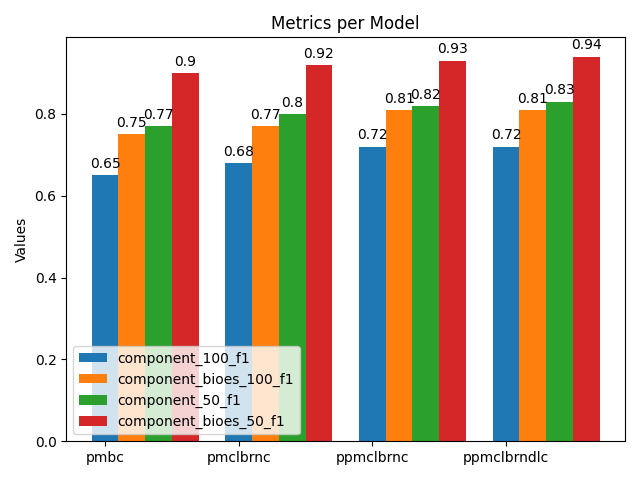
\includegraphics[scale=.4]{Graphics/persuasive_essays_all_linked_components.png}
		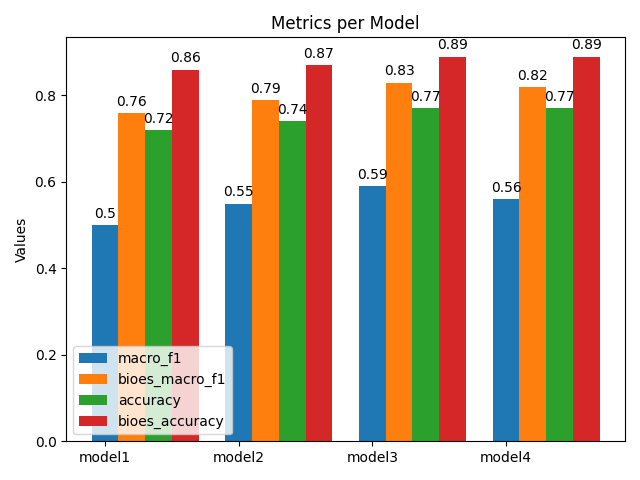
\includegraphics[scale=.4]{Graphics/persuasive_essays_all_linked_macro_micro_metrics.png}
	    \caption{Métricas del conjunto de pruebas de los modelos segmentadores.}\label{fig:test_segmenter_model_metrics}
	\end{center}
\end{figure}

El modelo seleccionado fue usado en el entrenamiento de los demás conjuntos de datos obteniendo los resultados mostrados
en Tabla \ref{table:test_metrics_segmenter} y Tabla \ref{table:test_bioes_metrics_segmenter}.

\begin{table}[h!]
	\begin{center}
		\scalebox{0.9}{
		\begin{tabular}{|c|c|c|c|c|c|} \hline
        Corpus		            & F1 Ponderado  & Macro F1	& \emph{Accuracy} & 100\%F1 & 50\%F1  	   \\ \hline
        Ensayos Argumentativos  & 0,76          & 0,56 		& 0,77		      & 0,72    & 0,83       \\ \hline
        CDCP		            & 0,65          & 0,45 		& 0,66		      & 0,61    & 0,68       \\ \hline
        AbsTRCT	                & 0,86          & 0,50 		& 0,87		      & 0,61    & 0,75       \\ \hline
        \end{tabular}
		}
	\caption{Métricas de las pruebas del segmentador de UDA.}\label{table:test_metrics_segmenter}
	\end{center}
\end{table}
\begin{table}[h!]
	\begin{center}
		\scalebox{0.9}{
		\begin{tabular}{|c|c|c|c|c|c|} \hline
        Corpus		            & F1 Ponderado  & Macro F1 & \emph{Accuracy} & 100\%F1 &  50\%F1   \\ \hline
        Ensayos Argumentativos  & 0,89          & 0,82	   & 0,89            & 0,81	   & 0,94 	   \\ \hline
        CDCP		            & 0,95          & 0,56	   & 0,96	         & 0,82	   & 0,93 	   \\ \hline
        AbsTRCT	                & 0,90          & 0,79	   & 0,91	         & 0,66	   & 0,82 	   \\ \hline
        \end{tabular}
		}
	\caption{Métricas BIOES de las pruebas del segmentador de UDA.}\label{table:test_bioes_metrics_segmenter}
	\end{center}
\end{table}

\subsection{Predictor de Enlaces}

Para el modelo se realizó un voto conjunto del ensamblado de 3 modelos, dado que el entrenamiento 
está basado en la aleatoriedad, se entrenan los modelos con los mismos datos obteniendo inferencias no
necesariamente iguales.
Para la selección del modelo se entrenaron diferentes variantes de arquitecturas e hiperparámetros, y 
al igual que en el segmentador de UDAs se realizó la selección del modelo que mejor se desempeñó en 
el conjunto de datos de Ensayos Argumentativos. De las variaciones surgieron las siguientes propuestas
(Tabla \ref{table:link_predictor_architecture_table}):

\begin{table}[h!]
	\begin{center}
		\scalebox{0.85}{
		\begin{tabular}{|c|c|c|c|c|c|c|} \hline
		Modelos   	 & Atención      & Pooling  & \emph{Dropout}   & Tasa de aprendizaje & Paciencia & Devolver mejores     \\ \hline
		Modelo 1	 & $\times$	     &  5       & 0,5               & 0,0015               & 10	      & $\checkmark$        \\ \hline
		Modelo 2	 & $\times$	 	 & 10       & 0,1               & 0,003                & 5	      & $\times$            \\ \hline
		Modelo 3	 & $\checkmark$	 &  1       & 0,1               & 0,003                & 5	      & $\times$            \\ \hline
		Modelo 4	 & $\checkmark$	 &  1       & 0,5               & 0,0015               & 10	      & $\checkmark$        \\ \hline
		\end{tabular}
		}
	\caption{Variantes de arquitectura de los modelos de predicción de enlaces.}\label{table:link_predictor_architecture_table}
	\end{center}
\end{table}

Las curvas de aprendizaje del proceso de entrenamiento de los modelos (Figura \ref{fig:link_prediction_model_loss}) 
muestran un nivel de sobreajuste 
elevado que disminuyen cuando el \emph{dropout} aumenta. Además, se observan valores de pérdida elevados lo que significa 
que al modelo le cuesta ajustarse de manera satisfactoria a los datos.

\begin{figure}[h!]
	\begin{center}
		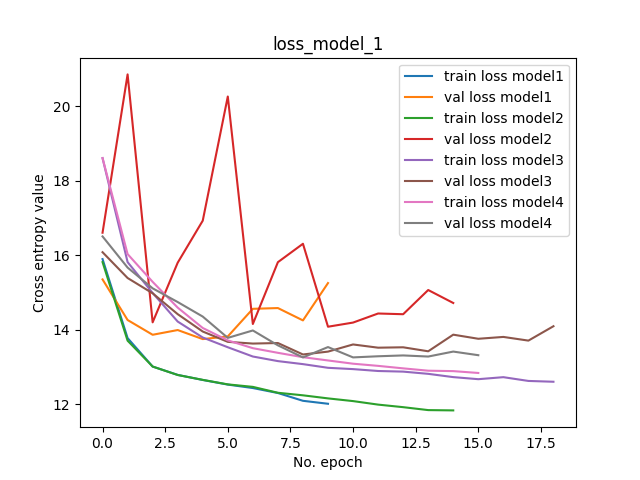
\includegraphics[scale=.7]{Graphics/persuassive_essays_all_linked_link_prediction_loss_model_1.png}
	    \caption{Curvas de aprendizaje de los modelos de predicción de enlaces.}\label{fig:link_prediction_model_loss}
	\end{center}
\end{figure}

Las métricas obtenidas por las diferentes versiones de los modelos 
(Figura \ref{fig:link_prediction_model_metrics}) 
muestran que el modelo 2 constituye una opción ligeramente superior en lo correspondiente a 
predicción de enlace a los otros modelos. Esos hiperparámetros
fueron utilizados para el entrenamiento con los demás conjuntos de datos.

\begin{figure}[h!]
	\begin{center}
		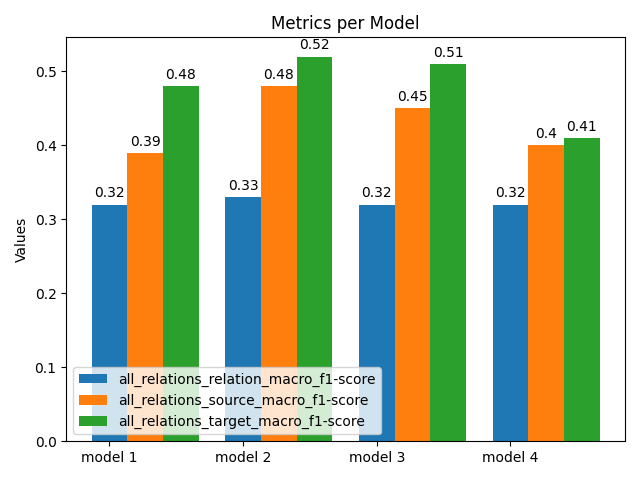
\includegraphics[scale=.4]{Graphics/persuasive_essays_all_linked_all_relation_f1_scores.png}
		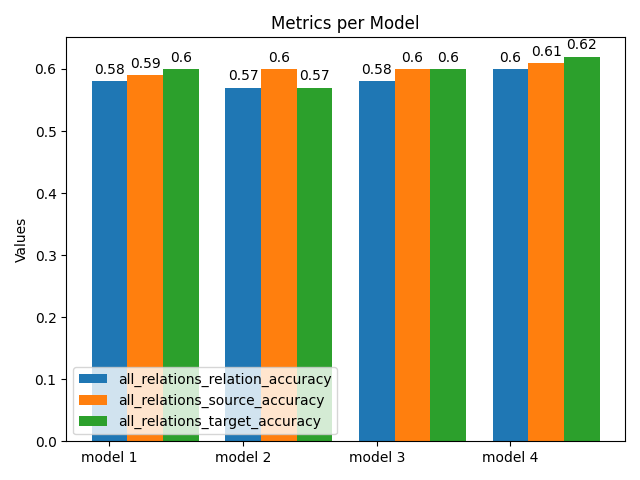
\includegraphics[scale=.4]{Graphics/persuasive_essays_all_linked_all_relation_accuracy.png}\\
		\text{a)$\qquad \qquad \qquad \qquad \qquad \qquad \qquad \qquad $b)}
	\end{center}
	\begin{center}
		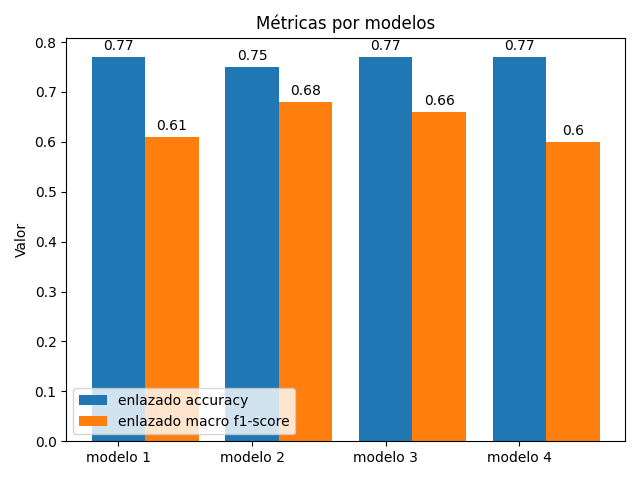
\includegraphics[scale=.4]{Graphics/persuasive_essays_all_linked_all_relation_linked.png}\\
		\text{c)}
	\end{center}
	\caption{Métricas F1 de la clasificación de enlace (a), \emph{accuracy} (b) y
			F1 de la predicción de enlace (c) de los modelos de predicción de enlaces.}
	\label{fig:link_prediction_model_metrics}
\end{figure}

En el entrenamiento del modelo en los demás conjuntos de datos se obtuvieron los resultados de las Tablas 
\ref{table:test_relation_metrics_link_predictor} y \ref{table:test_source_metrics_link_predictor}.

\begin{table}[h!]
	\begin{center}
		\scalebox{0.9}{
		\begin{tabular}{|c|c|c|c|c|} \hline
        Corpus		            & Macro F1 & \emph{Accuracy} & Macro F1 Enlace  & \emph{Accuracy} Enlace  \\ \hline
        Ensayos Argumentativos  & 0,33	   & 0,57            & 0,68	    		& 0,75	    		  	  \\ \hline
        CDCP		            & 0,37	   & 0,63	         & 0,79	    		& 0,68	    		  	  \\ \hline
        AbsTRCT	                & 0,39	   & 0,61	         & 0,83	    		& 0,74	    		  	  \\ \hline
        \end{tabular}
		}
	\caption{Métricas de predicción de relaciones de las pruebas del predictor de enlace.}\label{table:test_relation_metrics_link_predictor}
	\end{center}
\end{table}

\begin{table}[h!]
	\begin{center}
		\begin{tabular}{|c|c|c|c|} \hline
        Corpus		            & F1 Macro  & \emph{Accuracy} \\ \hline
        Ensayos Argumentativos  & 0,48       & 0,60             \\ \hline
        CDCP		            & 0,26       & 0,52	         \\ \hline
        AbsTRCT	                & 0,51       & 0,79	         \\ \hline
        \end{tabular}
	\caption{Métricas de predicción de fuente de las pruebas del predictor de enlace.}\label{table:test_source_metrics_link_predictor}
	\end{center}
\end{table}

\begin{table}[h!]
	\begin{center}
		\begin{tabular}{|c|c|c|c|} \hline
        Corpus		            & Macro F1 & \emph{Accuracy} \\ \hline
        Ensayos Argumentativos  & 0,52	   & 0,57             \\ \hline
        CDCP		            & 0,36	   & 0,54	         \\ \hline
        AbsTRCT	                & 0,53	   & 0,81	         \\ \hline
        \end{tabular}
	\caption{Métricas de predicción de objetivo de las pruebas del predictor de enlace.}\label{table:test_target_metrics_link_predictor}
	\end{center}
\end{table}

\subsection{Acoplamiento de los modelos}

Dado que la clasificación de UDAs es hecha tanto en el segmentador como en el predictor de enlaces, es necesaria 
la selección de cómo se va a desambiguar esta clasificación. En caso de seleccionar el predictor de enlaces como 
clasificador final, surgen varias cuestiones, como por ejemplo, que las UDAs pueden tomar varias clasificaciones o el
predictor no toma el contexto del texto completo en la clasificación. Aunque la primera puede ser corregida
mediante la selección de la clase más votada o algún otro criterio, la segunda presenta un mayor problema. Por
esto es seleccionada la clasificación del segmentador como etiqueta final para las UDAs y el predictor es usado para 
la tarea de extracción y clasificación de relaciones.

\subsection{Comparación con el estado del arte}

Las comparaciones se realizan por conjuntos de datos y se muestran las 
métricas indicadas por los autores de cada propuesta. Cada corpus y propuesta 
presenta características únicas que hacen que comparaciones directas sean 
difíciles de realizar, por lo tanto, la información brindada muestra una comparación 
cualitativa y no cuantitativa en la mayoría de los casos. 

Una de las principales dificultades está dada por el hecho de que las métricas calculadas son de la versión proyectada
al español, lo cual contribuye a variaciones en las etiquetas finales debido al lenguaje mismo 
o a errores en el proceso. Otros ejemplos en la dificultad de comparar las métricas se encuentra
en los enfoques tomados por las investigaciones anteriores a la hora de realizar las tareas.
En algunos casos la segmentación se presenta como una tarea de clasificación BIO, o simplemente 
se separan por oraciones y las clasifican en argumentativas o no. En el aspecto de clasificación
de las UDAs se emplean métodos como su clasificación independiente luego de ser extraída o su modelación
conjunta con la segmentación. En la extracción y clasificación de relaciones se observan técnicas de 
optimización de problemas enteros, clasificación por SVM o también probando los posibles enlaces dos 
a dos independientemente.

En la comparación de métodos se seleccionaron seis métricas que evalúan las diferentes 
tareas de la EA. La métrica BIOES F1 se refiere 
a la Macro F1 de la clasificación de las etiquetas BIOES, esta constituye una medida
que califica la tarea de segmentación de UDAs en el texto. La métrica Clas UDA F1 es 
calculada como la Macro F1 de las etiquetas BIOES junto con las etiquetas del tipo de 
UDA, medida que evalúa la tarea de clasificación de las UDAs. Rel Pred F1 es la medida 
Macro F1 de la predicción de enlaces y Rel Clas F1 la de la clasificación, estas 
son calculadas tomando en cuenta todos los pares seleccionados para el conjunto de 
datos. En la comparación $\checkmark$ significa que son directamente comparables,
$*$ que el método de comparación es el mismo, pero no son usados los mismos 
elementos para calcular la métrica, y $\times$ que la métrica no se encontraba disponible.

\begin{table}[h!]
	\begin{center}
		\scalebox{0.85}{
		\begin{tabular}{|c|c|c|c|c|c|} \hline
		Corpus		            & Propuesto  & \cite{stab2017parsing} & \cite{niculae2017argument} & \cite{galassi2021deep} \\ \hline
		BIOES F1 				& 0,82   	 & 0,85 $\checkmark$	  & $\times$        	       & $\times$				\\ \hline
		Clas UDA F1		        & 0,56	     & 0,82        			  & 0,77	    			   & 0,53					\\ \hline
		Rel Pred F1 			& 0,68   	 & 0,58        			  & 0,60			    	   & 0,36 *				   	\\ \hline
		Rel Clas F1 			& 0,33   	 & 0,70        			  & $\times$	    	       & 0,18 *				   	\\ \hline
		\end{tabular}
		}
	\caption{Métricas comparativas de Ensayos Persuasivos.}\label{table:comparative_test_essays_f1_metrics_segmenter}
	\end{center}
\end{table}
\begin{table}[h!]
	\begin{center}
		\begin{tabular}{|c|c|c|c|c|c|} \hline
		Corpus		            & Propuesto  & \cite{niculae2017argument} & \cite{galassi2021deep}  \\ \hline
		BIOES F1 				& 0,56  	 & $\times$        	       	  & $\times$				\\ \hline
		Clas UDA F1		        & 0,45	     & 0,73 				 	  & 0,79					\\ \hline
		Rel Pred F1				& 0,68   	 & 0,27			    	      & 0,30	*			   	\\ \hline
		Rel Clas F1				& 0,37   	 & $\times$	    	          & 0,15	*			   	\\ \hline
		\end{tabular}
	\caption{Métricas comparativas de CDCP.}\label{table:comparative_test_cdcp_f1_metrics_segmenter}
	\end{center}
\end{table}
\begin{table}[h!]
	\begin{center}
		\begin{tabular}{|c|c|c|c|c|c|} \hline
		Corpus		            & Propuesto  & \cite{mayer2020transformer} & \cite{galassi2021deep} \\ \hline
		BIOES F1 				& 0,79   	 & $\times$   				   & $\times$				\\ \hline
		Clas UDA F1		        & 0,50	     & 0,88	$\checkmark$		   & 0,91					\\ \hline
		Rel Pred F1 			& 0,74   	 & $\times$	   				   & 0,54 *				   	\\ \hline
		Rel Clas F1 			& 0,39   	 & 0,66  *	   				   & 0,70 *				   	\\ \hline
		\end{tabular}
	\caption{Métricas comparativas de AbsTRCT.}\label{table:comparative_test_abstrct_f1_metrics_segmenter}
	\end{center}
\end{table}

\section{Validación}

Dado que las estructuras argumentativas varían en su forma en cada corpus es complejo realizar un método que evalúe de forma 
justa los resultados obtenidos por los diferentes modelos de manera conjunta. Una variante sería anotar las cartas 
con los esquemas argumentativos presentes en los conjuntos de datos, esto constituye una labor en la que se requiere
personal experto y previo estudio y preparación, además de tiempo. El proceso que se lleva a cabo para realizar la 
validación consiste en un análisis cualitativo realizado a criterio del autor. Para esto se seleccionaron 15 pares 
de cartas, la carta original y la respuesta enviada a esta. Cada uno de estas 30 cartas fueron anotadas por los modelos entrenados en cada 
conjunto de datos y se realizó el análisis de calidad correspondiente. Los puntos por los que se llevó a cabo el análisis
se resumen en los siguientes:

\begin{itemize}
	\item ¿La UDA se extrajo correctamente?
	\item ¿La UDA se clasificó correctamente?
	\item ¿La relación se extrajo correctamente?
	\item ¿La relación se clasificó correctamente?
\end{itemize}

% \begin{itemize}
% 	\item Muchos falsos positivos en la predicción de enlaces, debido a la manera en la manera componente a componente que 
% 	se hacen
% 	\item En los textos en donde la segmentación es por oraciones, los puntos relacionados a otra acción que 
% 	no sea separar oraciones son seleccionados como separadores.
% 	\item La segmentación, se queda corta o larga?
% \end{itemize}

\subsection{Análisis de Ensayos Argumentativos}

% \begin{figure}[h!]
% 	\begin{center}
% 		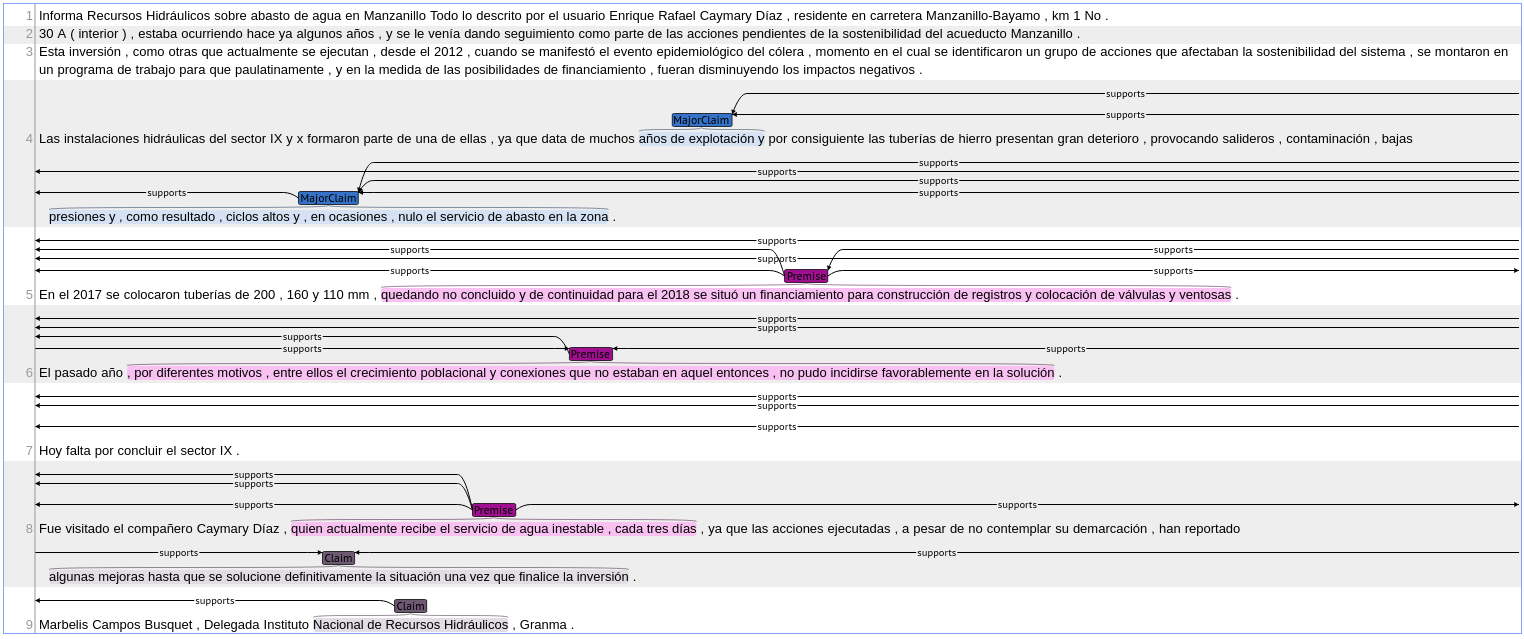
\includegraphics[scale=.4]{Graphics/persuasive_2019-01-25|informa-recursos-hidraulicos-sobre-abasto-de-agua-en-manzanillo|abasto-de-agua-en-manzanillo.png}
% 		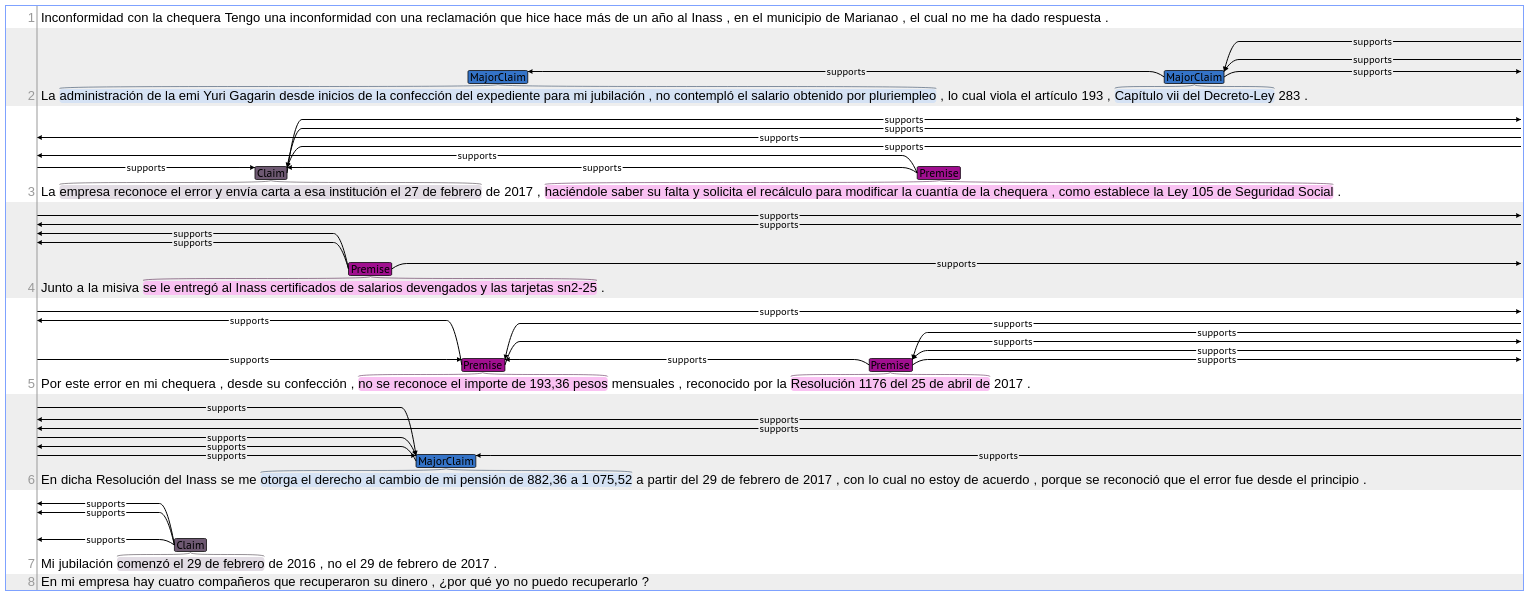
\includegraphics[scale=.4]{Graphics/persuasive_2019-03-22|inconformidad-con-la-chequera.png}
% 	    \caption{A}\label{fig:persuasive_granma_letters}
% 	\end{center}
% \end{figure}

Los ensayos argumentativos presentan una anotación de UDAs a un nivel de unidades de texto que pueden ser 
más pequeñas que oraciones y clasifican estas en las clases \emph{MajorClaim} (MC), \emph{Claim} (C) y \emph{Premise} 
(P). Las relaciones se clasifican en de \emph{supports} y \emph{attacks}. 

En general, se observa que se presentan problemas en la segmentación de UDAs debido al formato y dominio del texto.
Las cartas presentan una estrutura en donde al final se realiza una firma poniendo información acerca del remitente,
esta estructura no contribuye a la argumentación, pero el modelo en varias ocasiones detecta componentes en estas. 
Además de estos problemas de la estructura característica de la carta se encuentran otros. Entre los más 
encontrados se observa la extracción de supuestas UDAs que en su contenido no se encuentra un componente argumentativo, 
generalmente, estos elementos, si se expanden, pueden lograr establecer una mejor UDA.

Ejemplos malos:
\begin{itemize}
	\item \text{} [años de explotación y]$_{MC}$ 
	: Muy corto y no informativo. % 2019-01-25|informa-recursos-hidraulicos-sobre-abasto-de-agua-en-manzanillo|abasto-de-agua-en-manzanillo.txt.conll.link.conll.ann
	\item \text{} [en cada uno de los establecimientos de nuestra Cadena de Tiendas]$_{MC}$ 
	: Incompleto, mejora incorporando elementos de la izquierda (No a todos los productos con próxima fecha de vencimiento se le aplica rebaja de precios). % 2018-12-07|responde-trd-caribe-al-consumidor|a-proposito-de-la-proteccion-al-consumidor.txt.conll.link.conll.ann
	\item \text{} [Director División Grandes Centros]$_{MC}$ [TRD Caribe]$_{C}$ 
	: Mala clasificación y segmentación. %  2018-12-07|responde-trd-caribe-al-consumidor|a-proposito-de-la-proteccion-al-consumidor.txt.conll.link.conll.ann
	\item \text{} [Esperamos lo antes posible una solución]$_{P}$ 
	: En contexto, no contiene información que lo haga premisa % 2018-10-05|abasto-de-agua-en-manzanillo.txt.conll.link.conll.ann
	\item \text{} [no podemos permitir]$_{C}$ 
	: No establece una \emph{claim} % 2017-06-30|inass-reconoce-razon-de-ramiro-castellanos-por-inconformidad-con-trato-de-especialista-de-las-tunas|pregunta-quien-le-paga-su-jubilacion.txt.conll.link.conll.ann
\end{itemize}

Ejemplos buenos:
\begin{itemize}
	\item \text{} [no se le puede volver a despachar, tiene que ver a la administración (si está ahí en ese momento), 
	si no, regresar al día siguiente para que se le acredite lo sucedido]$_{MC}$ % 2021-02-26|inconvenientes-con-tarjetas-de-combustible-en-moneda-nacional.txt.conll.link.conll.ann
	\item \text{} [administración de la EMI Yuri Gagarin desde inicios de la confección del expediente para 
	mi jubilación, no contempló el salario obtenido por pluriempleo]$_{MC}$ % 2019-03-22|inconformidad-con-la-chequera.txt.conll.link.conll.ann
	\item pudiese [contribuir al ahorro de agua y la prestación de un mejor servicio]$_C$ % 2018-10-05|abasto-de-agua-en-manzanillo.txt.conll.link.conll.ann
	\item \text{} [es que estamos limitados de este servicio, y no desde hace un tiempo, es que nunca lo hemos tenido]$_P$ % 2018-05-18|sin-cobertura-en-guara-mayabeque.txt.conll.link.conll.ann
	\item \text{} [el número de carné de identidad que se encontraba en dicha base de datos correspondía a otra persona que
	fue reportada como fallecida]$_P$ % 2017-06-30|inass-reconoce-razon-de-ramiro-castellanos-por-inconformidad-con-trato-de-especialista-de-las-tunas|pregunta-quien-le-paga-su-jubilacion.txt.conll.link.conll.ann
\end{itemize}

Las relaciones anotadas por el modelo tienden a contener una gran cantidad de falsos positivos, además
dado que este conjunto de datos posee un gran desbalance en las etiquetas de las relaciones favoreciendo 
estas a las de \emph{supports}, el modelo no fue capaz de realizar anotaciones de \emph{attacks}, tanto en 
el conjunto de original de pruebas como en las cartas.

\subsection{Análisis de CDCP}

% \begin{figure}[h!]
% 	\begin{center}
% 		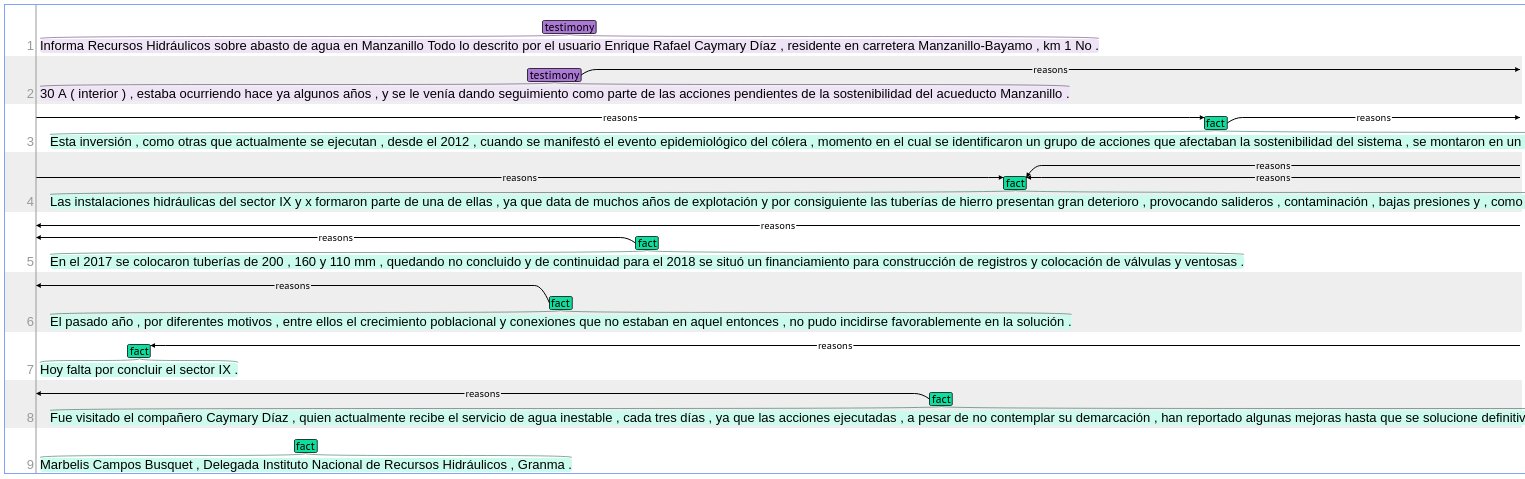
\includegraphics[scale=.4]{Graphics/cdcp_2019-01-25|informa-recursos-hidraulicos-sobre-abasto-de-agua-en-manzanillo|abasto-de-agua-en-manzanillo.png}
% 		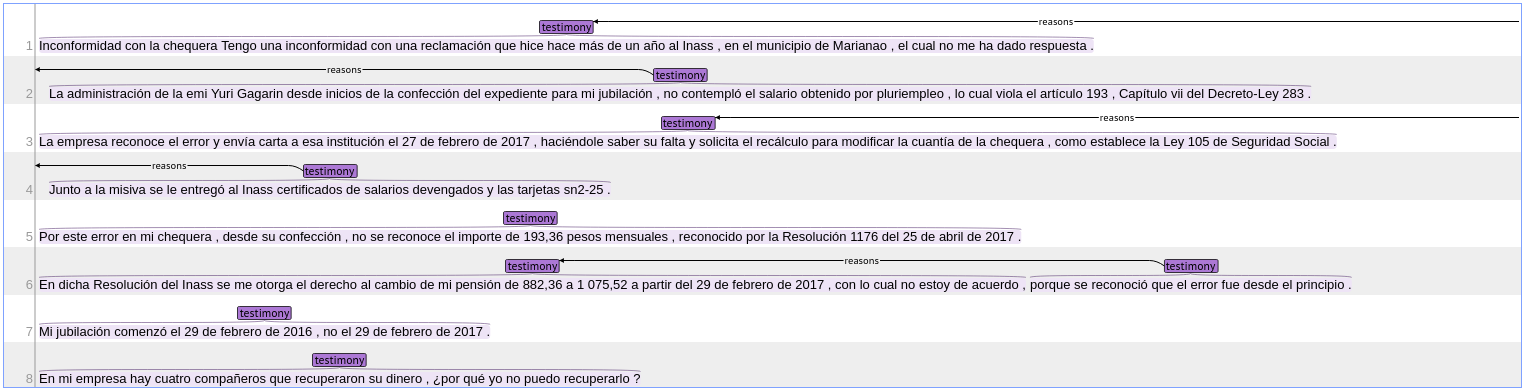
\includegraphics[scale=.4]{Graphics/cdcp_2019-03-22|inconformidad-con-la-chequera.png}
% 	    \caption{A}\label{fig:cdcp_granma_letters}
% 	\end{center}
% \end{figure}

CDCP realiza la segmentación de UDAs en la mayoría de las situaciones al separarlas por oraciones 
(solamente el 1\% de los tokens se encuentran fuera de una UDA),
estas son clasificadas en \emph{testimony} (T), \emph{fact} (F), \emph{policy} (P), \emph{reference} (R)
y \emph{value} (V). Las relaciones presentan dos tipos de relaciones \emph{evidences} y \emph{reasons}.

Los errores más comunes cometidos en la segmentación, dado el esquema utilizado, provienen del uso 
de signos de puntuación que no representan un cambio de oración, en estos casos se separa las UDA. También
existen errores de clasificación incorrecta, de, por ejemplo, \emph{testimony} que podrían ser \emph{fact}.

Ejemplos malos:
\begin{itemize}
	\item \text{} [\dots Bayamo, km 1 No.]$_T$ [30 A (interior), \dots]$_T$ 
	: Uso del \textbf{.} para abreviar número se toma como separador de UDA. % 2019-01-25|informa-recursos-hidraulicos-sobre-abasto-de-agua-en-manzanillo|abasto-de-agua-en-manzanillo.txt.conll.link.conll.ann
	\item \text{} [\dots ,desde el 1ro.]$_T$ [de marzo \dots]$_T$ 
	: Uso del \textbf{.} para abreviar primero se toma como separador de UDA. % 2019-05-24|le-retribuyen-la-diferencia-reclamada-de-su-pension|inconformidad-con-la-chequera.txt.conll.link.conll.ann
	\item \text{} [Junto a la misiva se le entregó al Inass certificados de salarios devengados y las tarjetas sn2-25.]$_T$ 
	: Se clasifica mejor como \emph{fact}. % 2019-03-22|inconformidad-con-la-chequera.txt.conll.link.conll.ann
	\item \text{} [Caridad Real Gutiérrez, Jefe de Trámites y Pensiones, Inass.]$_T$ 
	: Firma de la carta como elemento argumentaivo. % 2019-05-24|le-retribuyen-la-diferencia-reclamada-de-su-pension|inconformidad-con-la-chequera.txt.conll.link.conll.ann
\end{itemize}

Ejemplos buenos:
\begin{itemize}
	\item \text{} [En el 2017 se colocaron tuberías de 200, 160 y 110 mm, quedando no concluido y de 
	continuidad para el 2018 se situó un financiamiento para construcción de registros y colocación de 
	válvulas y ventosas.]$_F$ % 2019-01-25|informa-recursos-hidraulicos-sobre-abasto-de-agua-en-manzanillo|abasto-de-agua-en-manzanillo.txt.conll.link.conll.ann
	\item \text{} [Mi jubilación comenzó el 29 de febrero de 2016, no el 29 de febrero de 2017.]$_T$ % 2019-03-22|inconformidad-con-la-chequera.txt.conll.link.conll.ann
	\item \text{} [No se sabe cuánto queda, lo que obliga al cliente a estar haciendo cuentas constantemente.]$_F$ % 2021-05-07|servicentros-operan-diversos-medios-de-pago-electronicos|inconvenientes-con-tarjetas-de-combustible-en-moneda-nacional.txt.conll.link.conll.ann
\end{itemize}

Las relaciones presentes disminuyen en cantidad en comparación con lo visto en los textos anotados con el modelo 
entrenado con Ensayos Argumentativos. Prevaleciendo las relaciones de \emph{reasons}. A consideración del autor,
la cantidad de los falsos positivos son menores que el modelo de Ensayos Argumentativos.

\subsection{Análisis AbsTRCT}

% \begin{figure}[h!]
% 	\begin{center}
% 		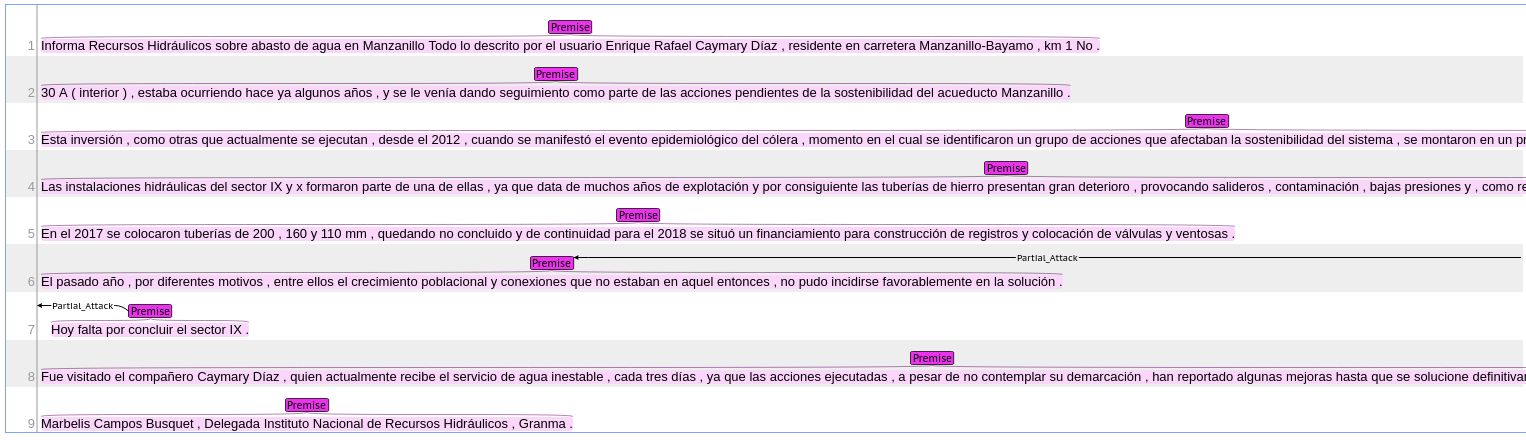
\includegraphics[scale=.4]{Graphics/abstrct_2019-01-25|informa-recursos-hidraulicos-sobre-abasto-de-agua-en-manzanillo|abasto-de-agua-en-manzanillo.png}
% 		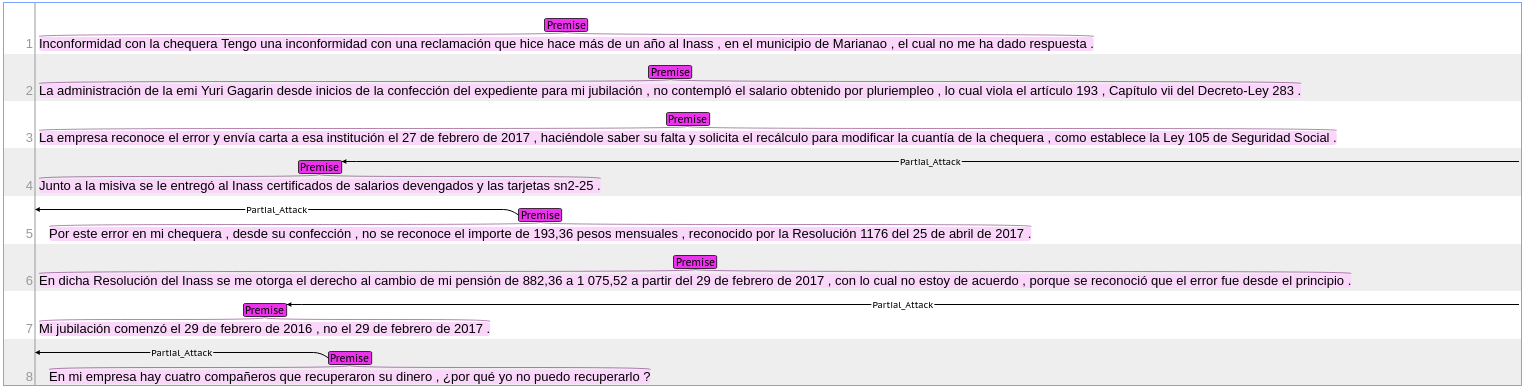
\includegraphics[scale=.4]{Graphics/abstrct_2019-03-22|inconformidad-con-la-chequera.png}
% 		\caption{A}\label{fig:abstrct_granma_letters}
% 	\end{center}
% \end{figure}

El conjunto de datos presenta un estilo de segmentación de UDAs en donde se anotan 
secciones de textos más grandes que en Ensayos Argumentativos, aunque no necesariamente 
todas las oraciones o la oración completa es considerada argumentativa. 
Estas se clasifican igual que Ensayos Argumentativos, aunque 
en este conjunto de datos se presenta un desbalance de etiquetas grande, favoreciendo 
a las \emph{Premise} y las \emph{Claim}, dejando sin representación casi a \emph{MajorClaim}
(menor del 1\% de las etiquetas BIOES), lo que trajo como consecuencia que el modelo no fuera 
capaz de diferenciar este tipo de UDA. Las relaciones se presentaron como \emph{partial-attack},
\emph{attack} y \emph{support}, influenciadas también por la poca cantidad de relaciones de \emph{attack}.

En la clasificación de UDAs se evidencia una gran cantidad de \emph{Premise}.

Ejemplos malos:
\begin{itemize}
	\item \text{} [\dots Calle 14, apto.]$_P$ [4 entre Zapata y 23, \dots]$_T$ 
	: Uso del \textbf{.} para abreviar apartamento se toma como separador de UDA. % 2017-07-07|parque-en-pleno-deterioro-en-plaza.txt.conll.link.conll.ann
	\item \text{} [, Director División Grandes Centros TRD Caribe.]$_C$ 
	: Mala clasificación con mala segmentación y detección de \emph{claim} en firma de carta. 
\end{itemize}

Ejemplos buenos:
\begin{itemize}
	\item \text{} [Esta situación pudo haberse evitado y no podemos permitir que hechos como este ocurran pues, 
	empañan la imagen de la institución que está destinada a brindar un servicio con calidad a la población en 
	general y en especial a los jubilados y pensionados.]$_P$ % 2017-06-30|inass-reconoce-razon-de-ramiro-castellanos-por-inconformidad-con-trato-de-especialista-de-las-tunas|pregunta-quien-le-paga-su-jubilacion.txt.conll.link.conll.ann
	\item \text{} [Esta respuesta considera sin razón la preocupación de un lector, 
	¿así debe terminar la inquietud de un ciudadano, que confía en las instituciones con que cuenta la 
	sociedad para enfrentar sus problemas?]$_C$ % 2017-05-12|cimex-se-dirige-a-limitado-fisico-motor|llamado-a-evaluar-situacion-de-piezas-y-baterias-para-equipos-motorizados-de-discapacitados.txt.conll.link.conll.ann
\end{itemize}

Las relaciones tienen la menor cantidad de elementos de los otros conjuntos de datos, proliferando
las relaciones de \emph{support}. En las clasificadas como \emph{partial-attack} se evidenció, a 
consideración del autor, una baja precisión. Por ejemplo 
[\emph{cierto que la responsabilidad es de todos, pero la institucional es de la Dirección de Comunales.}]
ataca a [\emph{Antonio Blanco, Director de Servicios Comunales Plaza,}].

\subsection{Resultados}

Se considera que el conjunto de datos CDCP se ajusta mejor a las características de las Cartas 
a la Dirección. Este presenta orígenes similares, es contenido generado por usuarios en una plataforma
web, y, por lo tanto, presenta un conjunto de etiquetas de UDAs que se ajustan más a lo observado 
en las cartas. También las cartas presentan un alto contenido argumentativo, por lo que marcar 
todas las oraciones como argumentativas no constituye una fuente grande de errores, aunque esta 
parte puede ser mejorada. Una desventaja de este esquema sobre otros es la carencia de una 
clasificación de las relaciones que implique un ataque, aunque esto se cubre con el hecho de 
que en los conjuntos en donde existen estas los resultados son bastante pobres en ese aspecto. La cantidad 
y calidad de relaciones, aunque tiene bastante espacio para mejorar, es aceptable dada la dificultad 
del problema en EA.

Con CDCP se obtiene una visión general de la argumentación, aunque si se desea obtener algo 
más específico podría considerarse el modelo de Ensayos Argumentativos. La ventaja de este 
modelo en la extracción y clasificación de UDA es que utiliza un conjunto de etiquetas que 
podría considerarse universal en la argumentación y además reduce el espacio de búsqueda de 
oraciones a segmentos de palabras, aunque estos puedan estar sujetos a errores. 

La versión de AbsTRCT constituye el modelo con menor rendimiento. La clasificación
de UDAs presenta una gran desproporción hacia \emph{Premise} dejando muchas \emph{Claim}
sin ser conrrectamente clasificadas. Sobre las relaciones muestra un nivel muy bajo de 
relaciones por documento, en relación a las que se podrían formar.
